\documentclass[compress,framenumber]{beamer}

\usetheme{UniversityofCambridge}

\usepackage{lipsum}
\usepackage{natbib}
\newcommand{\nat}{Nature}
\newcommand{\grl}{Geophysical Research Letters}
\newcommand{\gji}{Geophysical Journal International}
\newcommand{\jgr}{Journal of Geophysical Research (Solid Earth)}
\newcommand{\pepi}{Physics of the Earth and Planetary Interiors}
\newcommand{\epsl}{Earth and Planetary Science Letters}
\newcommand{\gca}{Geochimica et Cosmochimica Acta}
\newcommand{\cmp}{Contributions to Mineralogy and Petrology}
\newcommand{\bssa}{Bulletin of the Seismological Society of America}
\newcommand{\toms}{ACM Transactions on Mathematical Software}
\setbeamertemplate{bibliography item}[triangle]

\title{Marsquakes: A key to the structure and history of Mars' deep interior
\\$\,$}
\subtitle{GCB, May 11\textsuperscript{th} 2016}

\author{\hfill{Bob Myhill, Nick Teanby, James Wookey}} 
\begin{document}

% Title page
\begin{frame} 
\titlepage
\vspace{-1.0em}
\end{frame}


\section{Introduction}
% Motivation

\begin{frame}
  \frametitle{The Red Planet}
  \vspace{-2.0em}
  \begin{figure}
    \includegraphics[width=0.75\linewidth]{figures/mars_earth_comparison.pdf}
  \end{figure}

%Use these equations in one of the 'step' slides
\center{$P = \int_{r}^{R} \rho(P, T) g(r') dr' $, $g = 4\pi \frac{G}{r^2} \int_0^r
  \rho(P, T) r'^2 dr'$}
\end{frame}

\begin{frame}
  \frametitle{What do we know? Shallow chemistry}
  \vspace{-2.0em}
  \begin{figure}
    \includegraphics[width=0.85\linewidth]{figures/snc_meteorites.pdf}
  \end{figure}
\end{frame}

\begin{frame}
  \frametitle{What do we want to know? Interior chemistry}
  \vspace{-2.0em}
  \begin{figure}
    \includegraphics[width=0.80\linewidth]{figures/earth_section.pdf}
  \end{figure}
  \vspace{-1.0em}
  \hfill \copyright Johan Swanepoel, NASA
\end{frame}

\begin{frame}
  \frametitle{What do we want to know? Early history}
  \vspace{-2.0em}
  \begin{figure}
    \includegraphics[width=0.80\linewidth]{figures/impact.pdf}
  \end{figure}
  \hfill \copyright National Geographic
\end{frame}

\begin{frame}
  \frametitle{What do we want to know? Planetary evolution}
  \vspace{-2.0em}
  \begin{figure}
    \includegraphics[width=1.0\linewidth]{figures/MOLA_med_res.pdf}
  \end{figure}
\end{frame}

\section{The InSight Mission}

\begin{frame}
  \frametitle{How do we find this stuff out?}

\end{frame}

\begin{frame}
  \frametitle{Ray paths}
  \vspace{-4.0em}
  \begin{figure}
    \includegraphics[width=0.95\linewidth]{figures/ray_paths.pdf}
  \end{figure}
\end{frame}

\begin{frame}
  \frametitle{Ray paths}
  \vspace{-4.0em}
  \begin{figure}
    \includegraphics[width=0.95\linewidth]{figures/record_section.pdf}
  \end{figure}
\end{frame}

\begin{frame}
  \frametitle{Building a synthetic Mars}

  Step 2: Choose a composition and temperature gradient, find equilibrium density
  \vspace{-1.0em}
  \begin{figure}
    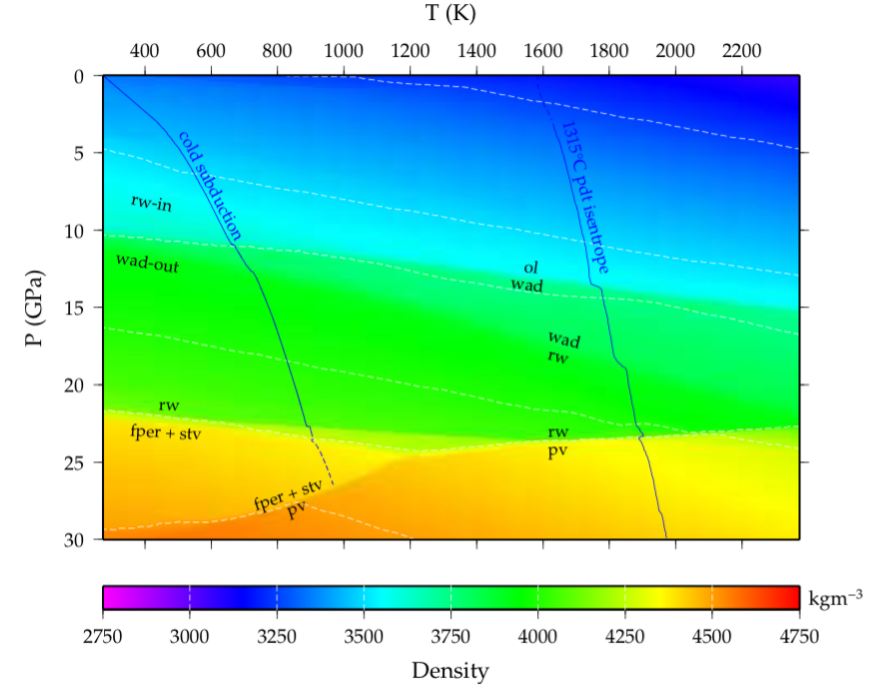
\includegraphics[width=0.7\linewidth]{figures/P_T_rho.pdf}
  \end{figure}
\end{frame}


\begin{frame}
  \frametitle{Building a synthetic Mars}
  Step 3: Build a planet with a core radius and density that fits
  Mars' mass and moment of inertia
  \vspace{-0.5em}
  \begin{figure}
    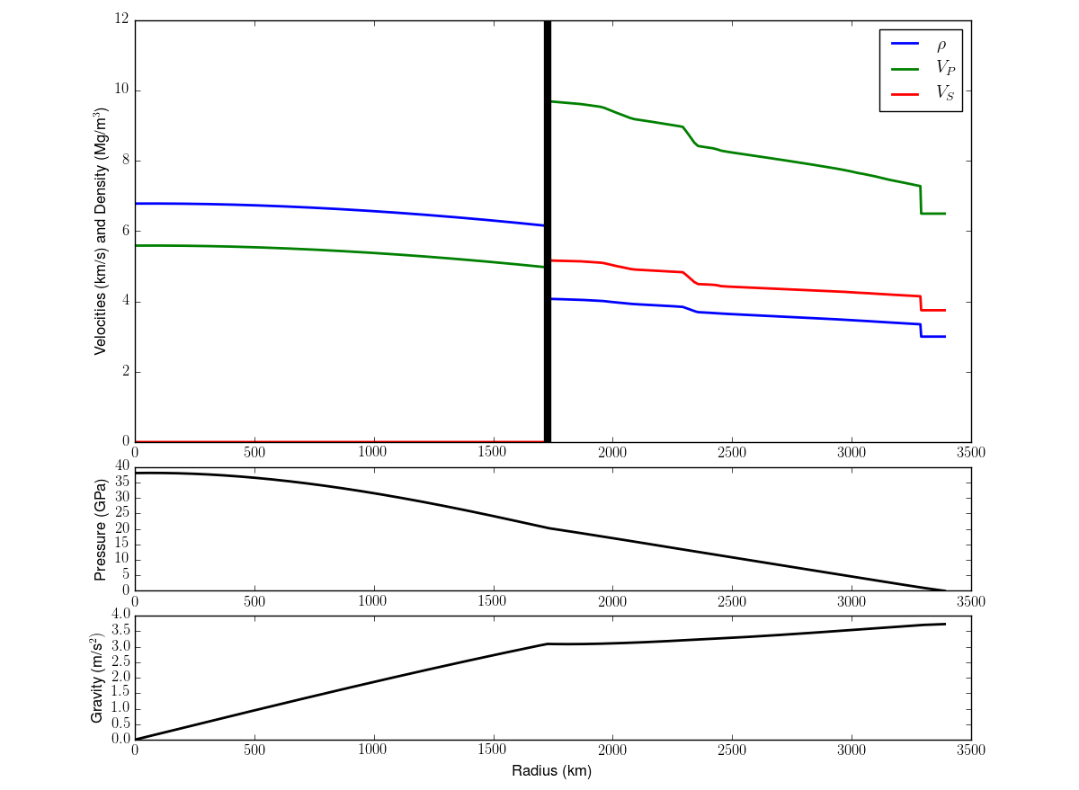
\includegraphics[width=0.7\linewidth]{figures/example_profile.pdf}
  \end{figure}
\end{frame}

\begin{frame}
  \frametitle{Building a synthetic Mars}
  Step 4: Add life \\(and hope that Curiosity doesn't kill it)
  \vspace{-0.5em}
  \begin{figure}
    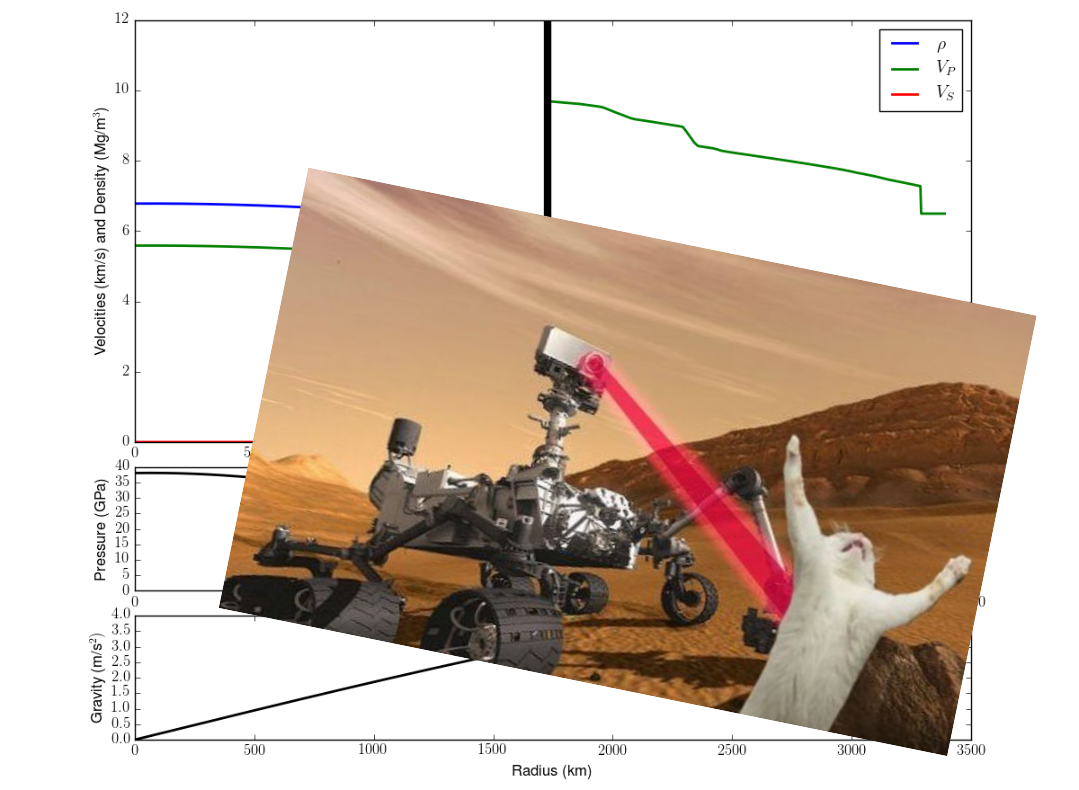
\includegraphics[width=0.7\linewidth]{figures/example_profile_with_life.pdf}
  \end{figure}
\end{frame}

\begin{frame}
  \frametitle{Core properties}
  \vspace{-1.em}
  \begin{figure}
    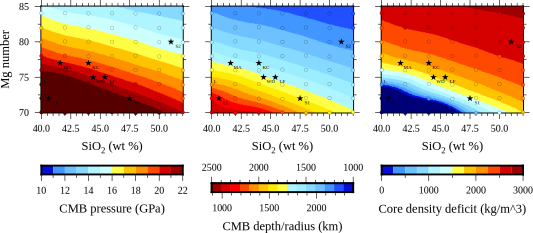
\includegraphics[width=0.95\linewidth]{figures/cmb_pressures_1673.pdf}
  \end{figure}
\end{frame}

\begin{frame}
  \frametitle{Making synthetic seismograms}
  Record section
  \vspace{-2.0em}
  \begin{figure}
    \includegraphics[width=0.65\linewidth]{figures/mars.pdf}
  \end{figure}
\end{frame}

\begin{frame}
  \frametitle{Weird and wonderful raypaths}
  Cross section
  \vspace{-2.0em}
  \begin{figure}
    \includegraphics[width=0.65\linewidth]{figures/mars.pdf}
  \end{figure}
\end{frame}

\begin{frame}
  \frametitle{Weird and wonderful raypaths}
  \vspace{-2.0em}
  \begin{figure}
    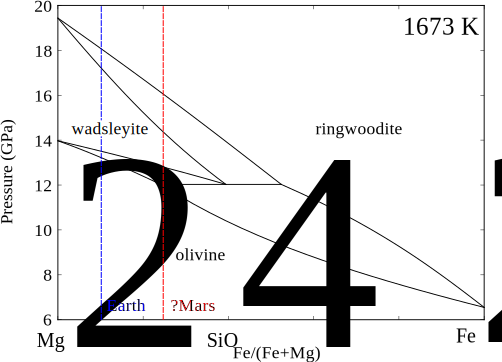
\includegraphics[width=0.65\linewidth]{figures/ol_wad_rw}
  \end{figure}
\end{frame}

\begin{frame}
  \frametitle{Constraining composition and temperature}
  \vspace{-2.0em}
  \begin{figure}
    \includegraphics[width=0.9\linewidth]{figures/PP_SP_differential_times.pdf}
  \end{figure}
\end{frame}

\begin{frame}
  \frametitle{Constraining core size without core phases?}
  \vspace{-2.0em}
  \begin{figure}
    \includegraphics[width=0.9\linewidth]{figures/PP_SP_differential_times_coresize.pdf}
  \end{figure}
\end{frame}

\section{Further work}

\begin{frame}
  \frametitle{Further work: Adding core-mantle interaction}
  \vspace{-2.0em}
  \begin{figure}
    \includegraphics[width=0.8\linewidth]{figures/ferric_depth_combined.pdf}
  \end{figure}
  \center{$Fe^{2+}$ (mineral) $\rightarrow$ $Fe^{3+}$ (mineral) + $Fe^{0}$ (sulfide melt)}
\end{frame}

\begin{frame}
  \frametitle{Further work: Adding core-mantle interaction}
  \vspace{-2.0em}
  \begin{figure}
    \includegraphics[width=0.75\linewidth]{figures/differentiation.pdf}
  \end{figure}
  \vspace{-2.0em}
  \hfill Mao et al., 2013
\end{frame}


\begin{frame}
  \frametitle{Further work: Receiver function modelling}
  \vspace{-2.0em}
  \begin{figure}
    \includegraphics[width=0.65\linewidth]{figures/r_fn.pdf}
  \end{figure}
  \hfill Ferris et al., 2003; Neumann et al., 2004 
\end{frame}

% Thanks
\begin{frame}
  \frametitle{You survived!}
  \vspace{-2.0em}
  \begin{figure}
    \includegraphics[width=0.75\linewidth]{figures/the_martian.pdf} 
  \end{figure}
   \center{Any questions?}
  %\vspace{-0.5em}
%\small{Thanks also to our stellar technicians at the BGI: Gerti Gollner, Stefan \"Ubelhack, Heinz Fischer, Hubert Schulze, Raphael Njul and Detlef Krau{\ss}e.}
\end{frame}




\end{document}
